\documentclass[11pt, letterpaper]{article}
\usepackage[utf8]{inputenc}
\usepackage[parfill]{parskip}
\usepackage{natbib}
\usepackage{graphicx}
\usepackage[font=small,labelfont=bf]{caption}

\newcommand{\A}{\mathcal{A}}
\newcommand{\Y}{\mathcal{Y}}

\title{The Label Bias Problem}
\author{Awni Hannun}
\date{\today}

\begin{document}
\maketitle

\begin{abstract}
Many sequence classification models suffer from the \emph{label bias problem}.
Understanding the label bias problem and when a certain model suffers from it
is subtle but is essential to understand the design of models like conditional
random fields and graph transformer networks.
\end{abstract}

\section{Introduction}

Many sequence classification models suffer from the \emph{label bias problem}.
Understanding the label bias problem and when a certain model suffers from it
is subtle but is essential to understand the design of models like conditional
random fields and graph transformer networks.

The label bias problem mostly shows up in discriminative sequence models. At
its worst, label bias can cause a model to completely ignore the current
observation when predicting the next label. How and why this happens is the
subject of this section. How to fix it is the subject of the next section.

Suppose we have a task like predicting the parts-of-speech for each word in a
sentence. For example, take the sentence ``the cat sat'' which consists of
the tokens \texttt{[the, cat, sat]}. We'd like our model to output the sequence
\texttt{[ARTICLE, NOUN, VERB]}.

A classic discriminative sequence model for solving this problem is the maximum
entropy Markov model (MEMM)~\citep{mccallum2000}. The graphical model for the
MEMM is shown in Figure~\ref{fig:memm}. Throughout, $X\!=\![x_1, \ldots, x_T]$
is the input or observation sequence and $Y\!=\![y_1, \ldots, y_T]$ is the
output or label sequence.

\begin{figure}
    \centering
    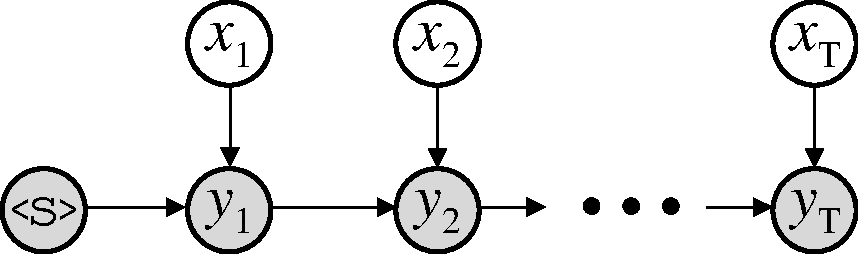
\includegraphics[width=0.7\textwidth]{figures/memm.pdf}
    \caption{The graphical model for the maximum entropy Markov model (MEMM).}
    \label{fig:memm}
\end{figure}

The MEMM makes two assumptions about the data. First, $y_t$ is conditionally
independent of all previous observations and labels given $x_t$ and $y_{t-1}$.
Second, the observations $x_t$ are independent of one another. The first
assumption is more central to the model while the second sometimes varies and
is easier to relax. These assumptions can be seen from the graphical model.
Mathematically, the model is written as

\begin{equation}
 p(Y \mid X) = \prod_{t=1}^T p(y_t \mid x_t, y_{t-1}).
\end{equation}

The probabilities are computed with a softmax:

\begin{equation}
 p(y_t \mid x_t, y_{t-1}) = \frac{e^{s(y_t, x_t, y_{t-1})}}{\sum_{i=1}^c e^{s(y_i, x_t, y_{t-1})}}
\end{equation}

where $c$ is the number of output classes and $s(y_t, x_t, y_{t-1})$ is a
scoring function which should give a higher score for $y_t$ which are likely to
be the correct label. Since we normalize over the set of possible output labels
at each time step, we say the model is \emph{locally normalized} and $p(y_t \mid
x_t, y_{t-1})$ are the \emph{local probabilities}. The distribution $p(Y \mid X)$ is
valid since summing over all possible $Y$ of length $T$ equals one, and all
the values are non-negative.

Let's return to our example of \texttt{[the, cat, sat]}. We can represent the
inference process on this sequence using a graph, as in
Figure~\ref{fig:memm_inf_norm}. The states (or nodes) represent the set of
possible labels. The transitions (or edges) represent the possible observations
along with the associated probabilities $p(y_t~\!\mid~\!x_t, y_{t-1})$.

\begin{figure}
    \centering
    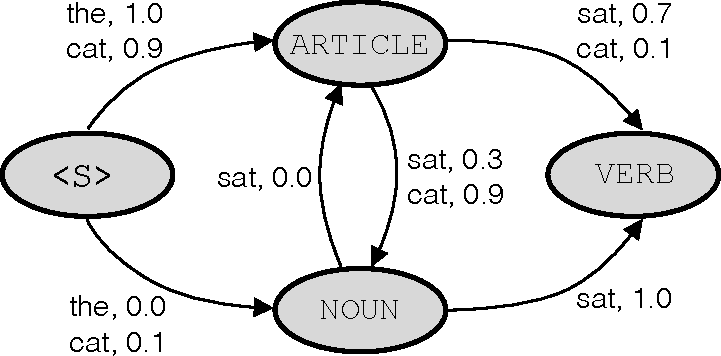
\includegraphics[width=0.7\textwidth]{figures/memm_inference_normalized.pdf}
    \caption{An inference graph for the MEMM with the label set
    \texttt{\{ARTICLE, NOUN, VERB\}}.  Each arc is labelled with the
    probability of transitioning to the corresponding state given the
    observation. The sum of the probabilities on arcs leaving a node for a
    given observation should sum to one. For simplicity not all observation,
    score pairs are pictured.}
    \label{fig:memm_inf_norm}
\end{figure}

To compute the probability of \texttt{[ARTICLE, NOUN, VERB]}, we just follow the
observations along each arc leading to the corresponding label. In this case
the probability would be $1.0\!\times\!0.9\!\times\!1.0$.

As another example, say we drop the article and just have the sequence
\texttt{[cat sat]}. While it's not a great sentence, the correct label should
be \texttt{[NOUN, VERB]}. However, if we follow the probabilities we see that
the score for \texttt{[ARTICLE, NOUN]} is $0.9\!\times\!0.3\!=\!0.27$ whereas
the score for \texttt{[NOUN, VERB]} is $0.1\!\times\!1.0\!=\!0.1$.

The model is not used to seeing \texttt{cat} at the start of a sentence, so the
scores leading from the start state are poorly calibrated. What we need is
information about how uncertain the model is for a given observation and
previous label pair. If the model has rarely seen the observation \texttt{cat}
from the starting node \texttt{<S>} then we want to know that, and it should be
included in the scores.

It's actually possible that the model did at some point implicitly store this
uncertainty information. However, by normalizing the outgoing scores for a
given observation, we are forcing this information to be discarded. Take a look
at the \emph{unnormalized} inference graph in Figure~\ref{fig:memm_inf_unnorm}.

\begin{figure}
    \centering
    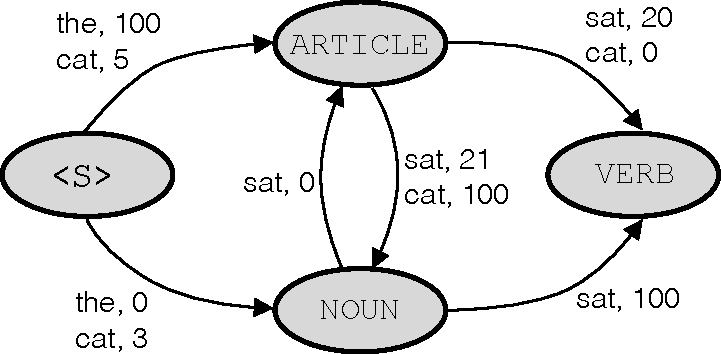
\includegraphics[width=0.7\textwidth]{figures/memm_inference_unnormalized.pdf}
    \caption{An \emph{unnormalized} inference graph for the MEMM with the label
    set \texttt{\{ARTICLE, NOUN, VERB\}}. Each arc is labelled with the score
    of transitioning to the corresponding state given the observation. For
    simplicity not all observation, score pairs are pictured.}
    \label{fig:memm_inf_unnorm}
\end{figure}

The unnormalized inference graph corresponds exactly to the normalized
inference graph when the scores are exponentiated and normalized. However, we
see something interesting here. The outgoing scores for \texttt{cat} from
\texttt{<S>} are small. Recall lower scores are worse. This means the model is
much less confident about the observation \texttt{cat} from the start state
than the observation \texttt{the} which has a score of $100$. This information
is completely erased when we normalize. That's one symptom of the label bias
problem.

Notice in the unnormalized graph, the score for \texttt{[ARTICLE, NOUN]} is $5 + 21 =
26$ while the score for \texttt{[NOUN, VERB]} is $3 + 100 = 103$. The right answer
gets a better score in the unnormalized graph! Note, we are adding scores here
instead of multiplying them because the unnormalized scores are in log-space.
In other words $p(y_t \mid x_t, y_{t-1}) \propto e^{s(y_t, x_t, y_{t-1})}$.

We can see the label bias problem quantitatively. This observation is due
to~\citet{denker1994}. Suppose our scoring function $s(y_t, x_t, y_{t-1})$
factorizes into the sum of two functions $f(y_t, x_t, y_{t-1})$ and $g(x_t,
y_{t-1})$. Suppose further that $f(\cdot)$ mostly cares about how good the
predicted label $y_t$ is given the observation $x_t$, whereas $g(\cdot)$ mostly
cares about how good the observation $x_t$ is given the previous label
$y_{t-1}$. If we compute the local probabilities using this factorization, we
get:
\begin{equation}
p(y_t \mid x_t, y_{t-1}) =
    \frac{e^{f(y_t, x_t, y_{t-1}) + g(x_t, y_{t-1})}}{
        \sum_{i=1}^c e^{f(y_i, x_t, y_{t-1}) + g(x_t, y_{t-1})}}
     = \frac{e^{f(y_t, x_t, y_{t-1})}}{\sum_{i=1}^c e^{f(y_i, x_t, y_{t-1})}}.
\end{equation}
The contribution of $g(\cdot)$ in the numerator and denominator cancels. This
causes all the information about how likely the observation is given the
previous state to be erased.


\subsection{Conservation of Score Mass}

The label bias problem results from a ``conservation of score
mass"~\citep{bottou1991}.  Conservation of score mass just says that the
outgoing scores from a state for a given observation are normalized. This means
that all of the incoming probability to a state must leave that state. An
observation can only dictate how much of the incoming probability to send
where. It cannot change the total amount of probability leaving the state. The
net result is any inference procedure will bias towards states with fewer
outgoing transitions.

Suppose we have three states, \texttt{A}, \texttt{B} and \texttt{C}, shown
in Figure~\ref{fig:trans}. State \texttt{A} has four outgoing (nonzero) transitions, state
\texttt{B} only has two and state \texttt{C} has just one. Suppose all three
states distribute probability mass equally among their successor states: $p(y_t
\mid x_t, y_{t-1})$ is uniform.

\begin{figure}
    \centering
    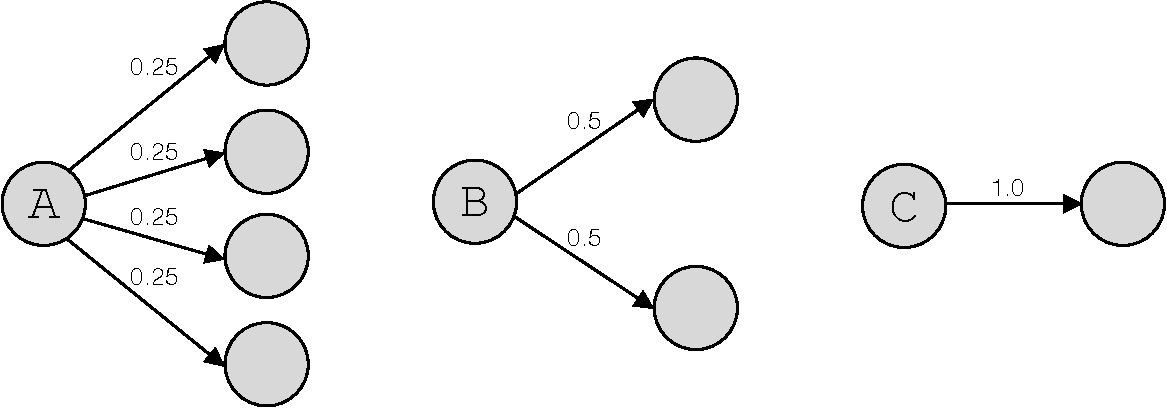
\includegraphics[width=0.7\textwidth]{figures/number_transitions.pdf}
    \caption{An example of three states, \texttt{A}, \texttt{B} and \texttt{C},
    which have uniform outgoing transition distributions. Label bias will cause
    the inference procedure to favor paths which go through state \texttt{C}.}
    \label{fig:trans}
\end{figure}

Neither state \texttt{A}, \texttt{B} nor \texttt{C} are doing anything useful
here, so we shouldn't prefer one over the other. But the inference procedure
will bias towards paths which go through state \texttt{C} over \texttt{B} and
\texttt{A}. Paths which go through \texttt{A} will be the least preferred. To
understand this, suppose that the same amount of probability arrives at the
three states. State \texttt{A} will decrease the probability mass for any path
by a factor of four, whereas state \texttt{B} will only decrease a given path's
score by a factor of two and state \texttt{C} won't penalize any path at all.
In every case the observation is ignored, but the state with the fewest
outgoing transitions is preferred.

Even if outgoing transitions from states \texttt{A} and \texttt{B} did not
ignore their observations, they would still reduce a paths score since the
probabilities aren't likely to be one. This would cause state \texttt{C} to be
preferred even though it always ignores it's observation.

\subsection{Entropy Bias}

In a less contrived setting where the distribution $p(y_t \mid x_t, y_{t-1})$
is not the same for every observation, our model will bias towards states which
have a low entropy distribution over next states given the previous state.
Note this is distinct from the distribution $p(y_t \mid x_t, y_{t-1})$ which
can have low entropy without directly causing label bias. However, if the
conditional distribution $p(y_t \mid y_{t-1})$ has low entropy then we are
potentially in trouble. For example, in the figure above, $p(y \mid
\texttt{B})$ has lower entropy than $p(y \mid \texttt{A})$.

Consider the three in Figure~\ref{fig:entropy}. In each case there are two possible
observations \texttt{a} and \texttt{b} and two possible successor states. We'd
like to know which one will introduce the most label bias into the model. To
answer that question, we need to make an assumption about the prior probability
over observations. Suppose that the prior, $p(x_t)$, is uniform (e.g. $p(a) =
p(b) = 0.5$).

\begin{figure}
    \centering
    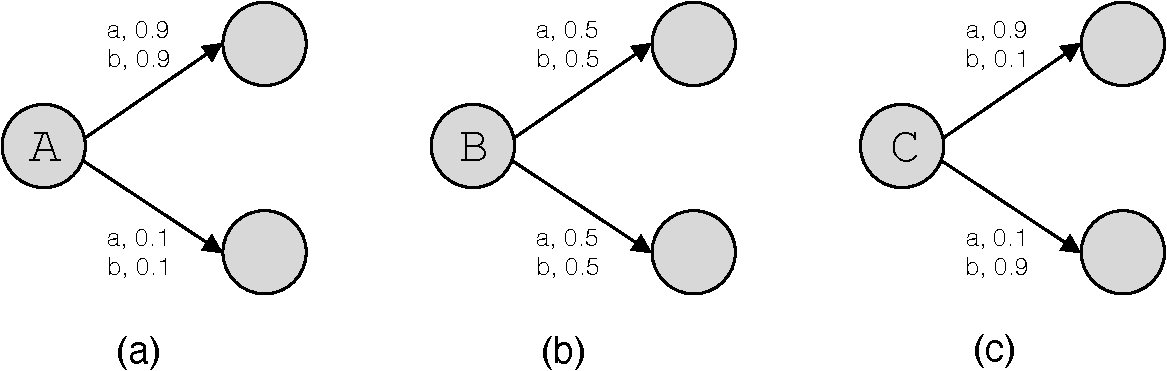
\includegraphics[width=0.7\textwidth]{figures/entropy_example.pdf}
    \caption{An example of three states, \texttt{A}, \texttt{B} and \texttt{C},
    each with two possible outgoing transitions. Each transition is labelled
    with the observation and probability pair for two observations, \texttt{a}
    and \texttt{b}.}
    \label{fig:entropy}
\end{figure}

We can calculate $p(y_t \mid y_{t-1})$ for any state since

\begin{equation}
p(y_t \mid y_{t-1}) = \sum_i p(y_t \mid x_i, y_{t-1}) p(x_i) = \frac{1}{n} \sum_i p(y_t \mid x_i, y_{t-1})
\end{equation}

where we used the fact that $p(x_t)$ is uniform and there are $n$ possible
observations. In our case $n\!~=\!~2$. Figure~\ref{fig:entropy_no_obs} shows
$p(y_t \mid y_{t-1})$ on the corresponding arc for each example.

\begin{figure}
    \centering
    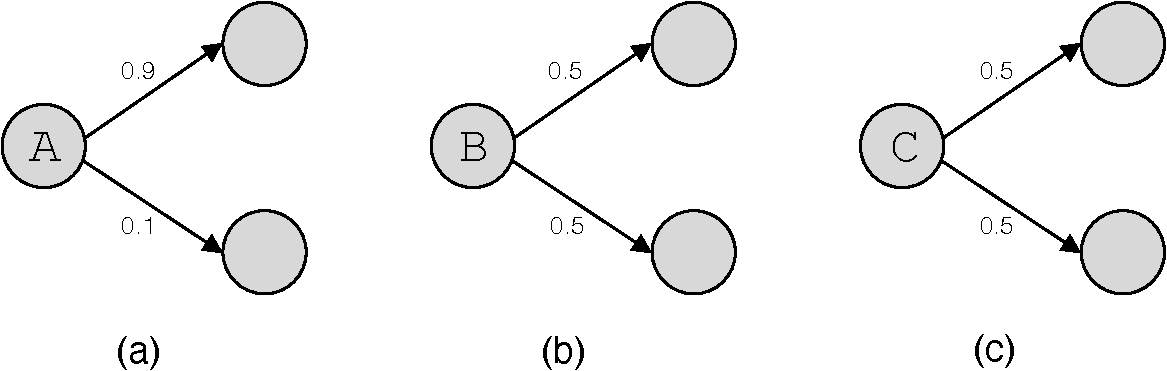
\includegraphics[width=0.7\textwidth]{figures/entropy_example_no_obs.pdf}
    \caption{An example of three states, \texttt{A}, \texttt{B} and \texttt{C},
    each with two possible outgoing transitions.  Each transition is labelled
    with the probability $p(y_t \mid y_{t-1})$ which are computed from the
    probabilities in the figure above.}
    \label{fig:entropy_no_obs}
\end{figure}

Case (a) has the lowest entropy transition distribution whereas case (b) and
(c) are equivalent. Intuitively, we expect case (a) to be worse than case (b)
since it biases towards the upper path, whereas (b) does not bias towards
either. However, case (c) is interesting. In case (c), the observation can have
a large effect on the outcome. While this effect might be wrong if the
probabilities are poorly calibrated, this case doesn't cause label bias more
than case (b) under the assumption of a uniform prior.

\subsection{Revising Past Mistakes}

Another description of the label bias problem is that it does not allow a model
to easily recover from past mistakes. This follows from the conservation of
score mass perspective. If the outgoing score mass of a path is conserved, then
at each transition the mass can only decrease. In the future, if a path
encounters new evidence which makes it very likely to be correct, it cannot
increase the path's score. The most this new evidence can do is to not decrease
the path's score by preserving all of the incoming mass for that path. So the
model's ability to promote a path given new evidence is limited even if we are
certain that the new observation makes this path the correct one.

\section{Overcoming the Label Bias Problem}

As we observed in the \texttt{[cat, sat]} example above, if we don't normalize
scores at each step, then the path scores can retain useful information. This
implies that we should avoid locally normalizing probabilities.

One option is that we don't normalize at all. Instead, when training, we simply
tune the model parameters to increase the score

\begin{equation}
    s(X, Y) = \sum_{t=1}^T s(y_t, x_t, y_{t-1})
\end{equation}

for every $(X, Y)$ pair in our training set. The problem with this is there is
no competition between possible outputs. This can result in the model
maximizing $s(Y, X)$ while completely ignoring its inputs. So we need some kind
of competition between outputs. If the score of one output goes up, then others
should feel pressure to go down.

This can be achieved with \emph{global normalization}. We compute the probability as
\begin{equation}
p(Y \mid X) = \frac{e^{\sum_{t=1}^T s(y_t, x_t, y_{t-1})}}{
    \sum_{Y^\prime \in \Y_T} e^{\sum_{t=1}^T s(y_t^\prime, x_t, y^\prime_{t-1})}}
\end{equation}
where $\Y_T$ is the set of all possible $Y$ of length $T$.  This is exactly a
linear chain conditional random field (CRF)~\citep{lafferty2001}. The graphical
model and hence dependency structure is the same as the MEMM in the previous
section. The only difference is how we normalize the scores for a given input.

With this normalization scheme, the label bias problem is no longer an issue.
In fact when performing inference, we need not normalize at all. The
normalization term is constant for a given $X$ and hence the ordering between
the possible $Y$ will be preserved without normalizing. What this means is that
the inference procedure operates on an unnormalized graph just like the one we
saw for the part-of-speech tagging example in the previous section.

Because transitions have unnormalized scores, they are free to affect the
overall path score anyway they please. If \texttt{cat} is very unlikely to
follow \texttt{<s>} the model can retain that information by keeping the scores
for all transitions out of \texttt{<s>} low. Then whenever we see \texttt{cat}
following the state \texttt{<s>}, the path score won't be affected much since
the model is uncertain of what the correct next label is.

This freedom from the label bias problem comes at a cost. Computing the
normalization term exactly is more expensive with a CRF than with an MEMM.
With an MEMM we normalize locally. Each local normalization costs
$\mathcal{O}(c)$ where $c$ is the number of classes, and we have to compute $T$
of them, so the total cost is $\mathcal{O}(cT)$. With a linear chain CRF, on
the other-hand, the total cost using an efficient dynamic programming algorithm
called the forward-backward algorithm, is $\mathcal{O}(c^2T)$~\citep{sutton2012}. If
$c$ is large this can be a major hit to training time. For more complex
structures where there can be longer-range dependencies between the outputs,
beam search is usually the only option to approximate the normalization
term~\citep{collobert2019}.

\section{A Brief History of the Label Bias Problem}

The first recorded observation of the label bias problem
was by~\citet{bottou1991}. The term ``label bias'' was coined in the seminal work
of~\citet{lafferty2001} introducing conditional random
fields. Solving the label bias problem was one of the
motivations for developing the CRF. The CRF was one of earliest discriminative
sequence models to give a principled solution to the label bias problem.

An even earlier sequence model which overcame the label bias problem was the
check reading system proposed by~\citet{denker1994}, though they did not use
the term label bias. This work motivated the graph transformer networks
of~\citet{bottou1997}. More references on graph transformer networks can be
found on Léon Bottou's webpage on structure learning
systems\footnote{https://leon.bottou.org/research/structured}.

\section{A Few Examples}

In this section we'll look at a few examples of models, some of which suffer
from label bias and some of which do not.

\subsection{Hidden Markov Model}

The hidden Markov model (HMM) is a generative model which makes two assumptions
about the data generating distribution. First, it assumes that the observation
$x_t$ is conditionally independent of all other $y$ and $x$ given the hidden
state (i.e. label) at time $t$, $y_t$. Second, the HMM makes the usual Markov
independence assumption that $y_t$ is conditionally independent of all previous
$y$ given $y_{t-1}$. In equations

\begin{equation}
p(X, Y) = p(y_0) \prod_{t=1}^T p(x_t \mid y_t) p(y_t \mid y_{t-1}).
\end{equation}

This is a very different model from the MEMM. It's generative, not
discriminative, so we estimate $p(X, Y)$ and not $p(Y \mid X)$. Interestingly,
the only difference between the graphical model for an HMM
(Figure~\ref{fig:hmm}) and the MEMM is the direction of the arrows between
$x_t$ and $y_t$.

\begin{figure}
    \centering
    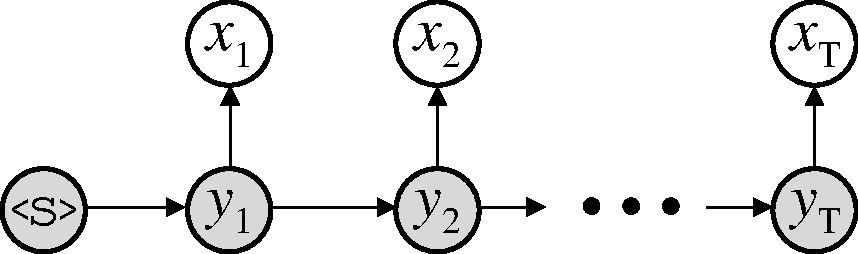
\includegraphics[width=0.7\textwidth]{figures/hmm.pdf}
    \caption{The graphical model for the hidden Markov model (HMM).}
    \label{fig:hmm}
\end{figure}

As a simple rule of thumb, generative models do not suffer from label bias. One
way to see this for the HMM specifically is to look at the corresponding
inference graph, as in Figure~\ref{fig:hmm_inference}.

\begin{figure}
    \centering
    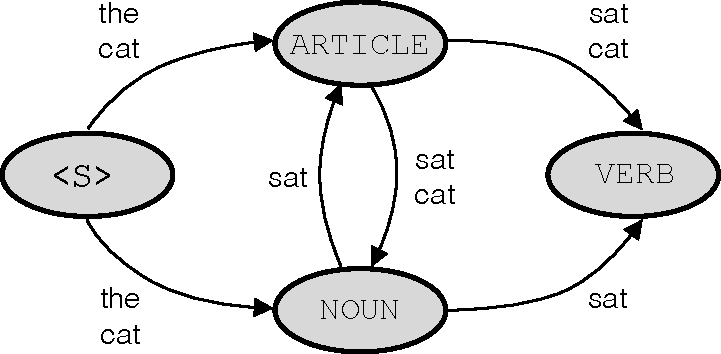
\includegraphics[width=0.7\textwidth]{figures/hmm_inference.pdf}
    \caption{An inference graph for the HMM with the label set
    \texttt{\{ARTICLE, NOUN, VERB\}}. The scores for the given observation on
    each arc are not shown.}
    \label{fig:hmm_inference}
\end{figure}

The scores on each edge associated with an observation are given by $p(x_t
\mid y_t) p(y_t \mid y_{t-1})$. In general the sum of these scores over all
possible next states is not required to be one:

\begin{equation}
\sum_{i=1}^c p(x_t \mid y_i) p(y_i \mid y_{t-1}) \ne 1.
\end{equation}

More importantly, the sum is not a constant, but can change depending on the
observation and the previous state. This implies that we do not have
conservation of score mass and hence label bias is not an issue.

\subsection{Sequence-to-sequence Models}

Sequence-to-sequence models with attention are very commonly used to label
sequences. These models are discriminative and compute the probability of an
output given an input using the chain rule

\begin{equation}
    p(Y \mid X) = \prod_{t=1}^T p(y_t \mid y_{<t}, X)
      \quad \textrm{where} \quad p(y_t \mid y_{<t}, X) \propto e^{s(y_t, y_{<t}, X)}.
\end{equation}

The score function $s(\cdot)$ is computed using a multi-layer neural network
with attention.

These models are locally normalized,

\begin{equation}
\sum_{i=1}^c p(y_i \mid y_{<t}, X) = 1,
\end{equation}

hence they can suffer from label bias. Whether or not this is an issue in
practice remains to be seen. Some attempts have been made to design globally
normalized versions of these models, though none are yet commonly
used~\citep{wiseman2016}.

\subsection{Connectionist Temporal Classification}

Connectionist Temporal Classification (CTC) is a discriminative sequence model
designed to solve problems where the correspondence between the input and
output sequence is unknown~\citep{graves2006} This includes problems like speech
and handwriting recognition among others. See \citet{hannun2017} for an
in-depth tutorial.

For a given input-output pair $(X, Y)$, CTC allows a set of alignments
$\A_{X,Y}$. We let $A\!=\![a_1, \ldots, a_T] \in \A_{X,Y}$ be one such alignment.
Note, $A$ has the same length as $X$, namely $T$. The probability of a sequence
$Y$ given an input $X$ can then be computed as

\begin{equation}
    p(Y \mid X) = \sum_{A \in \A_{X,Y}} \prod_{t=1}^T p(a_t \mid X)
     \quad \textrm{where} \quad p(a_t \mid X) \propto e^{s(a_t, X)}.
\end{equation}

Like sequence-to-sequence models with attention, the score function $s(\cdot)$
is usually computed with a multi-layer neural network. Notice that CTC assumes
the outputs $a_t$ are conditionally independent of one another given the input
$X$.

The CTC model is a special case in that it is both locally normalized and
globally normalized. Because of the conditional independence assumption, the
two are equivalent. At the level of an individual alignment, we have

\begin{equation}
p(A \mid X) = \prod_{t=1}^T \frac{e^{s_t(a_t, X)}}{\sum_{i=1}^c e^{s_t(a_i, X)}}
    = \frac{\prod_{t=1}^T e^{s_t(a_t, X)}}{\prod_{t=1}^T \sum_{i=1}^c e^{s_t(a_i, X)}}.
\end{equation}

We can rewrite the denominator using the fact that

\begin{equation}
\prod_{j=1}^m \sum_{i_j=1}^n a_{i_j} =
    \left(\sum_{i_1=1}^n a_{i_1}\right) \ldots \left(\sum_{i_m=1}^n a_{i_m}\right)
    = \sum_{i_1=1}^m \ldots \sum_{i_m=1}^n \prod_{j=1}^m a_{i_j}
\end{equation}

to get

\begin{equation}
p(A \mid X) = \frac{e^{\sum_{t=1}^T s_t(a_t, X)}}{\sum_{A^\prime} e^{\sum_{t=1}^T s_t(a^\prime_t, X)}}.
\end{equation}

Used on its own, CTC does not suffer from label bias. There are a couple of
ways to see this. First, as we described, CTC is globally normalized at the
level of an alignment and label bias results from local normalization.

Second, the conditional independence assumption made by CTC removes label bias.
If the next state prediction does not depend on any previous state, then there
is no label bias. The model acts as if the transition probabilities $p(y_t \mid
y_{t-1})$ are uniform and the same for all $y_{t-1}$. This means the entropies
of these distributions are all the same and maximal.

The model does have conservation of score mass in the sense that $\sum_{i=1}^c
p(y_i \mid X) = 1$. However, new evidence can arbitrarily influence the
plausibility of a given path. The model can favor paths which have a certain
label at a given time step by giving the corresponding $p(y_t \mid X)$ a value
close to one. This will in turn make all paths which do not predict $y_t$ have
scores very close to zero. However, the expressiveness of the model is also limited
since it cannot select for paths based on previously predicted labels.

\bibliographystyle{plainnat}
\bibliography{refs}

\end{document}
